\chapter{Strip transmission line medium for TEM wave propagation}\label{theory}

\indent The development of waveguide and other transmission lines for the low-loss power transmission at high frequencies was one of the early milestones in microwave engineering. Transmission in early RF and microwave systems relied on waveguides, two-wire lines, and coaxial lines. Waveguides have the advantage of high power-handling capability and low loss, but are bulky and expensive, especially at low frequencies. Two-wire lines are inexpensive, but lack shielding. Coaxial lines are shielded but are a difficult medium to fabricate complex microwave components. Planar transmission lines provide an alternative, in the form of stripline, microstrip lines, slotlines, coplanar waveguides, and several other types of related geometries. Such transmission lines are compact, low in cost, and capable of being easily integrated with active circuit devices, such as diodes and transistors, to form microwave integrated circuits.
\\
\indent In this chapter a transmission line that consist of two or more conductors and support transverse electromagnetic (TEM) waves is considered. A transmission line can be characterized by the propagation constant, the attenuation constant, and the characteristic impedance \cite{balanis} which are derived here to provide theoretical background for further analysis.
\\
\indent Even though, transmission lines are lossy structures due to finite conductivity and/or lossy dielectric, these losses are usually small and for many practical problems may be neglected. However, when e.g. high power circuits with low line attenuation are necessary, resonant circuits in which very high quality factor are of need or low-noise feeding networks for active circuits are required, the effect of loss must be taken into account. Therefore, a lossy transmission line is considered here to allow for inclusion of the loss effects on a transmission line behavior \cite{pozar}.


\section{Wave propagation in a lossy transmission line}\label{th:lossy}

\indent A one dimensional section of transmission line shown schematically in Fig. \ref{th:fig1a} as a two-wire line representation can be considered in terms of propagating voltage and current waves along $z$-axis. At a distance $z$, there is current $I(z)$ traveling through each wire, and there is voltage difference $V(z)$ between the wires. To calculate their distance and time relations, a transmission line model shown in Fig. \ref{th:fig1b} can be used. The section of line of infinitesimal length $\Delta z$ is modeled as a lumped-element circuit, where $L$, $R$, $C$, $G$, are per-unit-length quantities defined as follows:

\begin{itemize}[nosep]
\item $L$ is a series inductance per unit length, for both conductors, in (H/m), representing the total self-inductance of two conductors;
\item $R$ is a series resistance per unit length, for both conductors, in ($\Omega$/m), representing the resistance due to the finite conductivity of the individual conductors;
\item $C$ is a shunt capacitance per unit length, in (F/m), representing the total self-capacitance due to the close proximity of the two conductors;
\item $G$ is a shunt conductance per unit length, in (S/m), representing the dielectric loss in the material between the conductors.
\end{itemize}

\noindent A finite length of a transmission line can be seen as a cascade of sections of the form shown in Fig. \ref{th:fig1b}. 

%%%%%%%%%%%%%%%%%%%%%%%%%%%%%%%%%%%%%%%%%%%%%%%%%%%%%%%%%%%%%
\begin{figure}[H]
\centering
\begin{tabular}{c}
\subfloat[] { 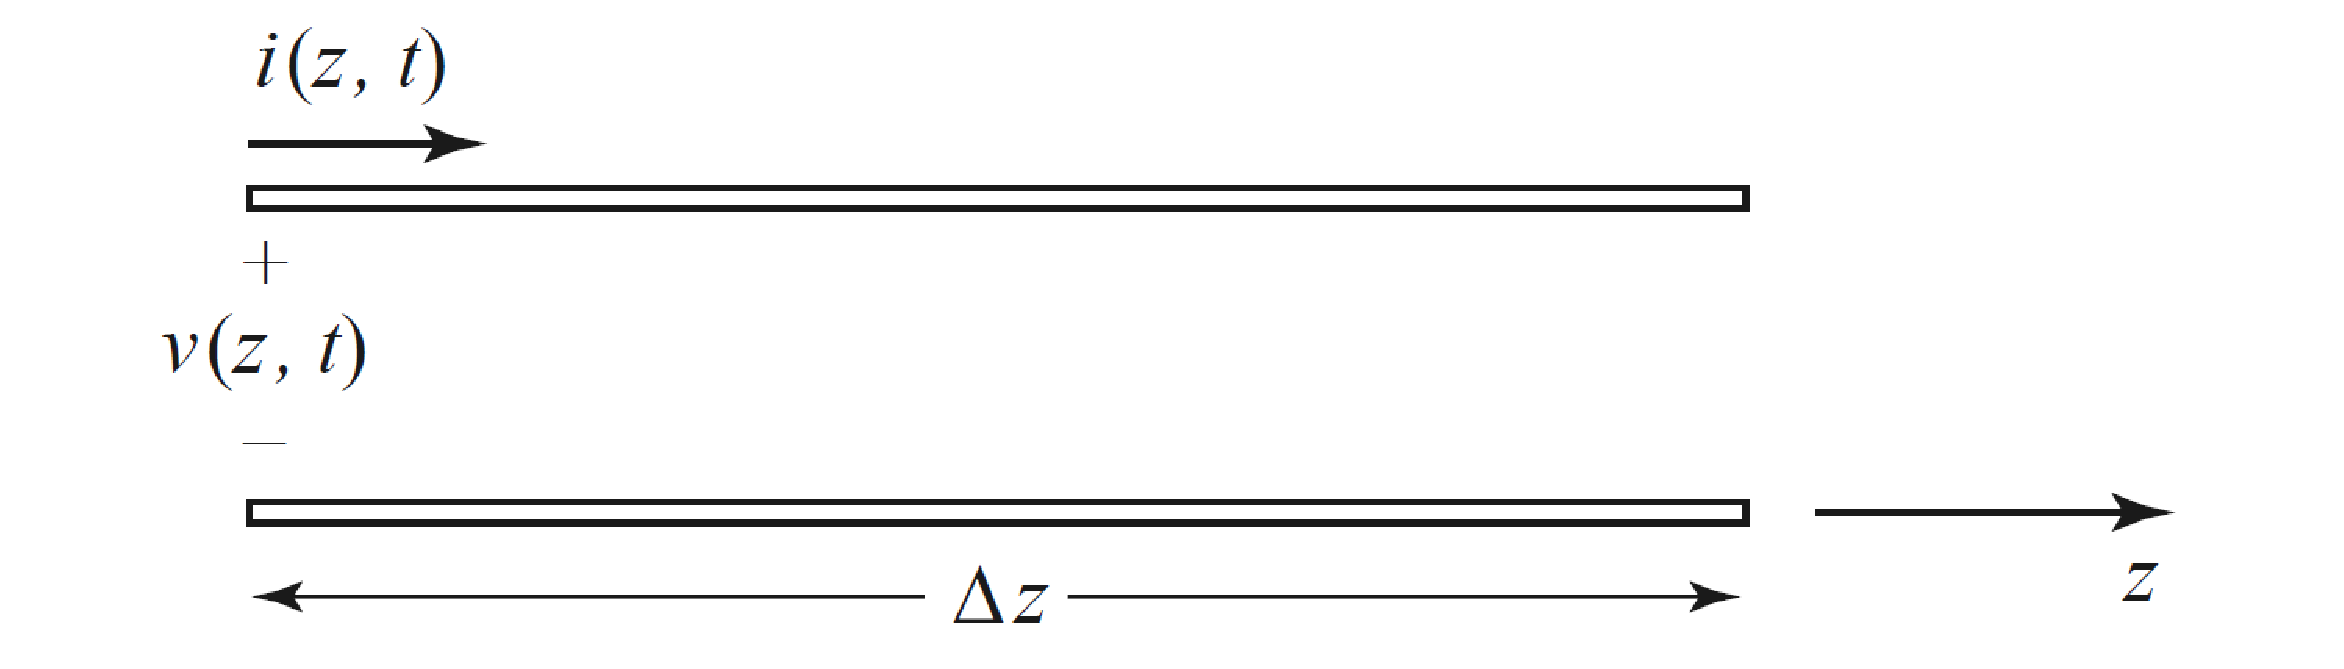
\includegraphics[scale=0.25]{chapter_2/fig1a.eps}\label{th:fig1a} }
\\
\subfloat[] { 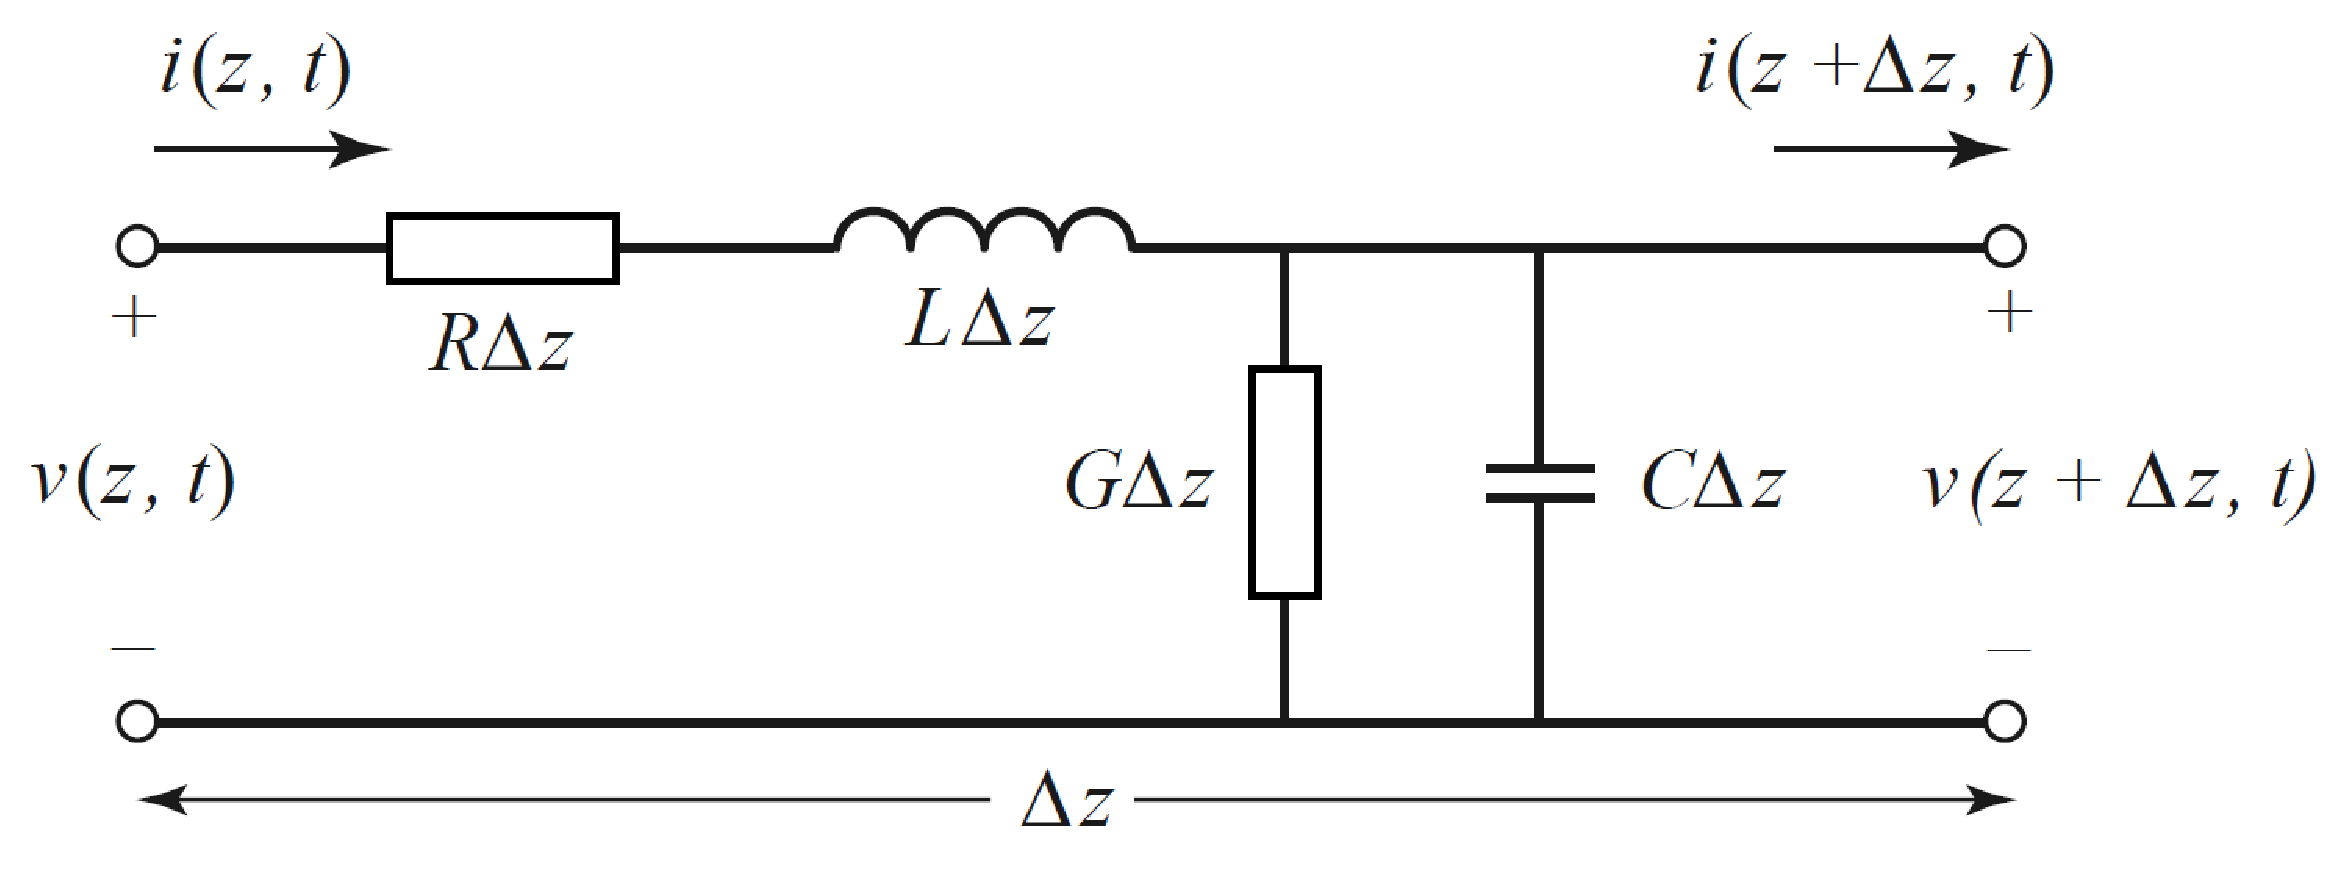
\includegraphics[scale=0.25]{chapter_2/fig1b.eps}\label{th:fig1b} }
\\
\end{tabular}
\caption{Definitions of voltage and current (a) together with lumped-element equivalent circuit for an incremental length of transmission line (b)}
\label{th:fig1}
\end{figure}
%%%%%%%%%%%%%%%%%%%%%%%%%%%%%%%%%%%%%%%%%%%%%%%%%%%%%%%%%%%%%

\indent From the circuit shown in Fig. \ref{th:fig1b}, Kirchhoff’s voltage law can be applied to give:

\begin{subequations}
\begin{equation}\label{th:eq1a}
v(z,t)-R\Delta zi(z,t)-L\Delta z\frac{\partial i(z,t)}{\partial t}-v(z+\Delta z,t)=0,
\end{equation}
and Kirchhoff’s current law leads to:
\begin{equation}\label{th:eq1b}
i(z,t)-G\Delta zv(z+\Delta z,t)-C\Delta z\frac{\partial v(z+\Delta z,t)}{\partial t}-i(z+\Delta z,t)=0.
\end{equation}
\end{subequations}

\noindent Dividing \ref{th:eq1a} and \ref{th:eq1b} by $\Delta z$ and taking the limit as $\Delta z \rightarrow 0$ gives the following differential equations:

\begin{subequations}
\begin{equation}\label{th:eq2a}
\frac{\partial v(z,t)}{\partial z}=-Ri(z,t)-L\frac{\partial i(z,t)}{\partial t},
\end{equation}
\begin{equation}\label{th:eq2b}
\frac{\partial i(z,t)}{\partial z}=-Gv(z,t)-C\frac{\partial v(z,t)}{\partial t}.
\end{equation}
\end{subequations}

\noindent These are the time domain form of the transmission line equations, also known as the telegrapher equations.
\\
\indent For the sinusoidal steady-state condition, with cosine-based phasors, \ref{th:eq2a} and \ref{th:eq2b} simplify to:

\begin{subequations}\label{th:eq3} 
\begin{equation}\label{th:eq3a}
\frac{dV(z)}{dz}=-(R+j\omega L)I(z),
\end{equation}
\begin{equation}\label{th:eq3b}
\frac{dI(z)}{dz}=-(G+j\omega C)V(z).
\end{equation}
\end{subequations}

\indent Following, the two equations \ref{th:eq3a} and \ref{th:eq3b} can be solved simultaneously to give wave equations for $V(z)$ and $I(z)$:

\begin{subequations}\label{th:eq4}
\begin{equation}\label{th:eq4a}
\frac{d^{2}V(z)}{dz^{2}}-\gamma ^{2}V(z)=0,
\end{equation}
\begin{equation}\label{th:eq4b}
\frac{d^{2}I(z)}{dz^{2}}-\gamma ^{2}I(z)=0,
\end{equation}
\end{subequations}

\begin{equation}\label{th:eq5}
\gamma = \alpha + j\beta = \sqrt{(R+j\omega L)(G+j\omega C)}
\end{equation}

\noindent where \ref{th:eq5} is the complex propagation constant, which is a function of frequency. Traveling wave solutions to \ref{th:eq4} can be found as:

\begin{subequations}\label{th:eq6}
\begin{equation}\label{th:eq6a}
V(z)=V_{o}^{+}e^{-\gamma z}+V_{o}^{-}e^{\gamma z},
\end{equation}
\begin{equation}\label{th:eq6b}
I(z)=I_{o}^{+}e^{-\gamma z}+I_{o}^{-}e^{\gamma z},
\end{equation}
\end{subequations}

\noindent where the $e^{-\gamma z}$ term represents wave propagation in the $+z$ direction, and the $e^{\gamma z}$ term represents wave propagation in the $-z$ direction. Applying \ref{th:eq3a} to the voltage of \ref{th:eq6a} gives the current on the line:

\begin{equation}\label{th:eq7}
I(z)=\frac{\gamma}{R+j\omega L}(V_{o}^{+}e^{-\gamma z}+V_{o}^{-}e^{\gamma z}).
\end{equation}

\indent Comparison of \ref{th:eq7} with \ref{th:eq6b} shows that the characteristic impedance $Z_{0}$, can be defined as:

\begin{equation}\label{th:eq8}
Z_{0}=\frac{R+j\omega L}{\gamma}=\sqrt{\frac{R+j\omega L}{G+j\omega C}},
\end{equation}

\noindent to relate the voltage and current on the line as follows:

\begin{equation}\label{th:eq9}
\frac{V_{o}^{+}}{I_{o}^{+}}=Z_{0}=\frac{-V_{o}^{-}}{I_{o}^{-}}.
\end{equation}

\noindent Then \ref{th:eq6b} can be rewritten in the following form:

\begin{equation}\label{th:eq10}
I(z)=\frac{V_{o}^{+}}{Z_{0}}e^{-\gamma z}-\frac{V_{o}^{-}}{Z_{0}}e^{\gamma z}.
\end{equation}

\indent Converting back to the time domain, we can express the voltage waveform as:

\begin{equation}\label{th:eq11}
v(z,t)=|V_{o}^{+}|cos(\omega t-\beta z +\phi ^{+})e^{-\alpha z}+|V_{o}^{-}|cos(\omega t+\beta z +\phi ^{-})e^{\alpha z},
\end{equation}

\noindent where $\phi ^{\pm }$ is the phase angle of the complex voltage $V_{o}^{\pm }$. Moreover, the wavelength on the line is

\begin{equation}\label{th:eq12}
\lambda = \frac{2\pi }{\beta },
\end{equation}

\noindent while the phase and group velocities are

\begin{subequations}\label{th:eq13}
\begin{equation}\label{th:eq13a}
v_{p} = \frac{\omega }{\beta }=\lambda f=\frac{1}{\sqrt{\epsilon \mu }},
\end{equation}
\begin{equation}\label{th:eq13b}
v_{g} = \frac{\partial \omega }{\partial \beta }.
\end{equation}
\end{subequations}

\indent The phase velocity $v_p$ corresponds to the propagation of a perturbation, i.e. it is the velocity at which a fixed phase point on the wave travels, while the group velocity $v_g$ corresponds to the propagation of energy. In a conventional medium, where permittivity $\epsilon $ and permability $\mu $ are greater than 0, the Electric field–Magnetic field–propagation constant ($\overline{E},\overline{H},\overline{\beta }$) builds the right-handed (RH) triad, therefore $v_p$ and $v_g$ are positive values describing a forward-wave propagation, outward from the source. However, if a medium would feature $\epsilon ,\mu$ < 0, a left-handed (LH) triad is build \cite{caloz}. Thus, as frequency is always a positive quantity, the phase velocity in a LH medium would be opposite to the phase velocity in a RH medium. Moreover, because $\beta $ is known to be positive in a RH medium, it would be negative in a LH medium, hence phase as related to the phase velocity, propagates backwards to the source in the opposite direction than that of power as being related to the group velocity.

\section{Power loss in a terminated lossy transmission line}\label{th:terminated}
%\section{Attenuation constant on a terminated lossy transmission line}\label{th:terminated}

The voltage and current wave propagating along a length $l$ of a lossy transmission line terminated by the impedance $Z_{L}$, as shown in Fig. \ref{th:fig2}, with propagation constant $\beta $ is attenuated at a constant rate of $\alpha $. Thus, $\gamma = \alpha + j\beta $ is complex, however, it is assumed that loss is small, so that $Z_{0}$ is approximately real. The actual power delivered to the load can be determined using the analysis given below.

%%%%%%%%%%%%%%%%%%%%%%%%%%%%%%%%%%%%%%%%%%%%%%%%%%%%%%%%%%%%%
\begin{figure}[H]
\centering
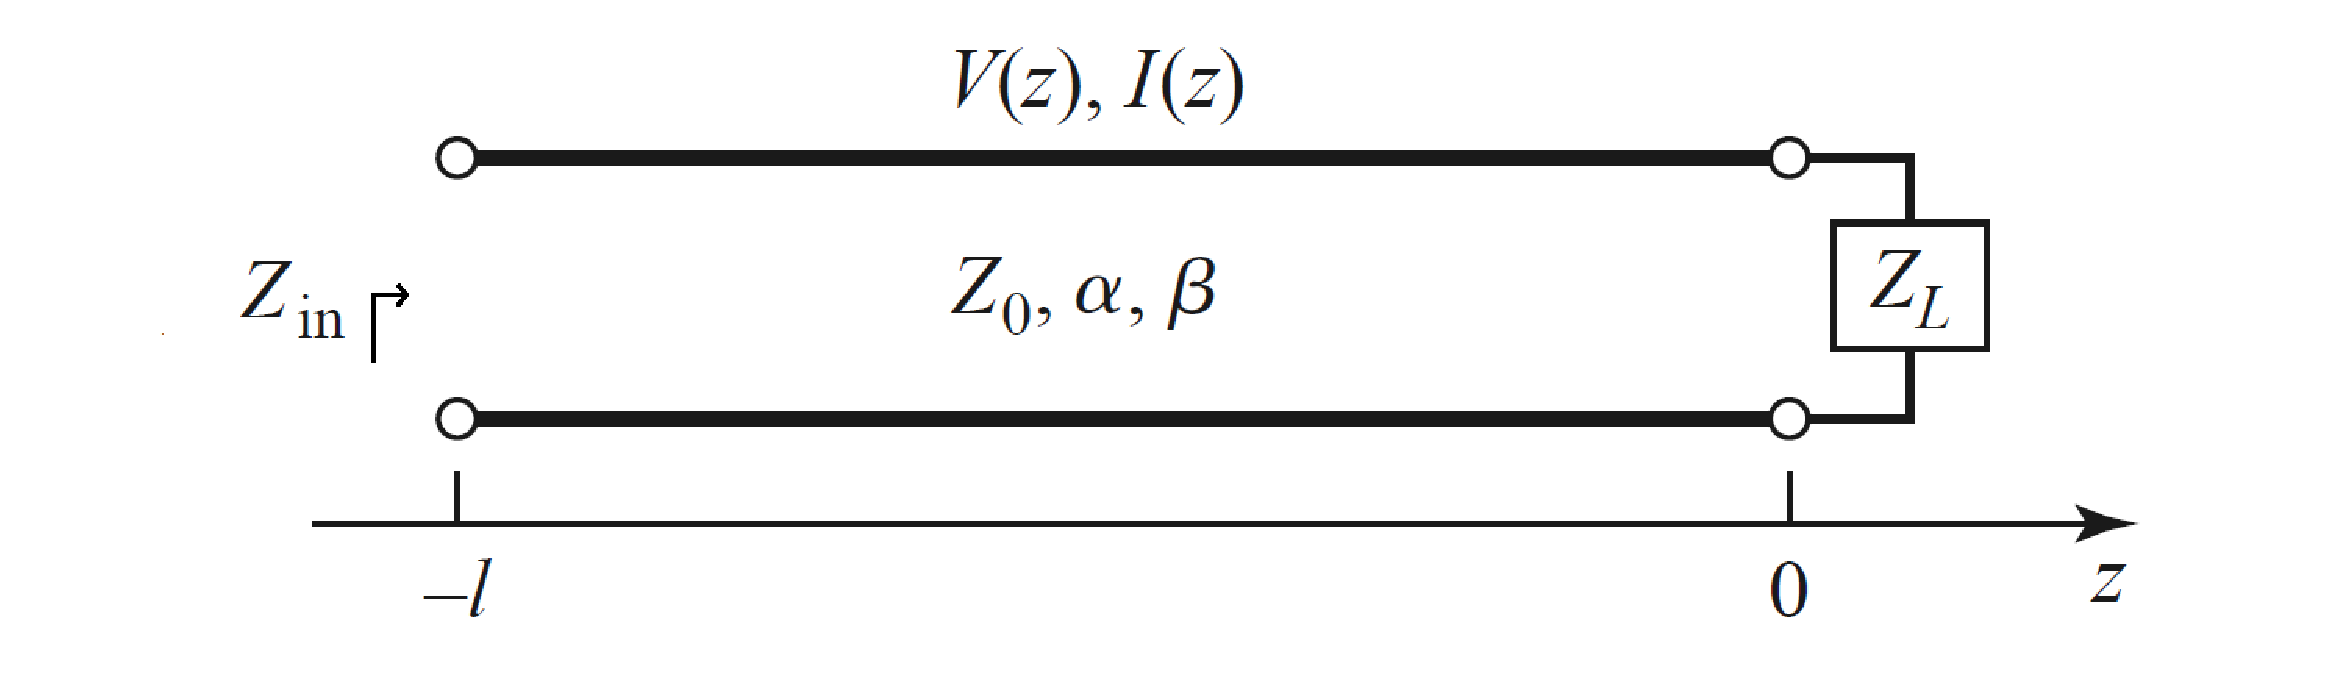
\includegraphics[scale=0.25]{chapter_2/fig2.eps}
\caption{A lossy transmission line terminated by the impedance $Z_{L}$.}
\label{th:fig2}
\end{figure}
%%%%%%%%%%%%%%%%%%%%%%%%%%%%%%%%%%%%%%%%%%%%%%%%%%%%%%%%%%%%%

\indent The voltage and current wave can be expressed as:

\begin{subequations}\label{th:eq14}
\begin{equation}\label{th:eq14a}
V(z)=V_{o}^{+}(e^{-\gamma z}+\Gamma e^{\gamma z}),
\end{equation}
\begin{equation}\label{th:eq14b}
I(z)=\frac{V_{o}^{+}}{Z_{0}}(e^{-\gamma z}-\Gamma e^{\gamma z}),
\end{equation}
\end{subequations}

\noindent where $\Gamma $ is the reflection coefficient of the load and $V_{o}^{+}$ is the incident
voltage amplitude referenced at $z$ = 0. The reflection coefficient at a distance $l$ from the load is:

\begin{equation}\label{th:eq15}
\Gamma (l)=\Gamma e^{-2j\beta l}e^{-2\alpha l}=\Gamma e^{-2\gamma l},
\end{equation}

\noindent The input impedance $Z_{in}$ at a distance $l$ from the load is then:

\begin{equation}\label{th:eq16}
Z_{in}=\frac{V(-l)}{I(-l)}=Z_{0}\frac{Z_{L}+Z_{0}tanh\gamma l}{Z_{0}+Z_{L}tanh\gamma l}.
\end{equation}

\noindent The power delivered to the input of the terminated line at $z = -l$ can be calculated as:

\begin{equation}\label{th:eq17}
P_{in}=\frac{1}{2}Re\left\{ V(-l)I^{*}(-l) \right\}=\frac{|V_{o}^{+}|^2}{2Z_{0}}(e^{2\alpha l}-|\Gamma |^{2}e^{-2\alpha l})=\frac{|V_{o}^{+}|^2}{2Z_{0}}(1-|\Gamma (l)|^{2})e^{2\alpha l},
\end{equation}

\noindent where \ref{th:eq14} has been used for $V(-l)$ and $I(-l)$. The power actually delivered to the
load is

\begin{equation}\label{th:eq18}
P_{L}=\frac{1}{2}Re\left\{ V(0)I^{*}(0) \right\}=\frac{|V_{o}^{+}|^{2}}{2Z_{0}}(1-|\Gamma |^{2}). 
\end{equation}

\noindent The difference in these powers corresponds to the power lost in the line:

\begin{equation}\label{th:eq19}
P_{loss}=P_{in}-P_{L}=\frac{|V_{o}^{+}|}{2Z_{0}}\left[ (e^{2\alpha l}-1)+|\Gamma |^{2}(1-e^{2\alpha l}) \right].
\end{equation}

\noindent The first term in \ref{th:eq19} accounts for the power loss of the incident wave, while the second
term accounts for the power loss of the reflected wave. It must be noted that both terms increase as $\alpha $
increases.

\indent The attenuation constant of a low-loss line can be found with a common and useful technique called the perturbation method. The method relies on the fields of the lossless line, with the assumption that the fields of the lossy line are not greatly different. Such an approach allows to avoid the use of the transmission line parameters $L$, $R$, $C$, $G$.

\indent The power flow along a lossy transmission line, in the absence of reflections, is of the form:

\begin{equation}\label{th:eq20}
P_{z}=P_{o}e^{-2\alpha z},
\end{equation}

\noindent where $P_{o}$ is the power at the $z$ = 0 plane and $\alpha $ is the attenuation constant we wish to determine. The power loss per unit length along the line can be defined as:

\begin{equation}\label{th:eq21}
P_{l}=-\frac{\partial{P}}{\partial{z}}=2\alpha P_{o}e^{-2\alpha z}=2\alpha P(z),
\end{equation}

\noindent where the negative sign on the derivative was introduced so that $P_{l}$ would be a positive quantity. From \ref{th:eq21}, the attenuation constant can be determined as:

\begin{equation}\label{th:eq22}
\alpha =\frac{P_{l}(z)}{2P(z)}=\frac{P_{l}(z=0)}{2P_{o}}.
\end{equation}

\noindent The equation \ref{th:eq22} states that $\alpha $ can be determined from the power on the line $P_{o}$ and the power loss per unit length of line $P_{l}$. It is important to realize that $P_{l}$ can be computed from the fields of the lossless line and can account for both conductor loss %[using (1.131) dopisać]
and dielectric loss. % [using (1.92) dopisać].
\\
\indent The power loss in a good conductor can be accurately and simply calculated in terms of the surface resistance of the conductor $R_{S}$ and the surface current $\bar{J}_{S}$, or tangential magnetic field $\bar{H}_{S}$:
% $\alpha = 1/\sigma _{S}

\begin{equation}\label{th:eq23}
P_{lcond} =\frac{R_{s}}{2}\int_{S}|\bar{J}_{S}|^{2}ds=\frac{R_{s}}{2}\int_{S}|\bar{H}_{t}|^{2}ds
\end{equation}

\noindent where $\int_{S}$ denotes a surface integral over the conductor surface and $R_{S}$ is determined from material conductivity $\sigma $ and current skin depth $\delta _{S}$:

\begin{equation}\label{th:eq24}
R_{S} =\frac{1}{\sigma \delta _{S}}=\sqrt{\frac{\omega \mu}{2\sigma}}.
\end{equation}

\indent On the other hand, the time averaged power dissipated in the volume $V$ of the isotropic, homogeneous, linear medium due to conductivity, dielectric, and magnetic losses can be determined as:

\begin{equation}\label{th:eq25}
P_{ldiel} =\frac{\sigma}{2}\int_{V}|\bar{E}|^{2}+\frac{\omega}{2}\int_{V}(\epsilon ^{''}|\bar{E}|^{2}+\mu ^{''}|\bar{H}|^{2})dv
\end{equation}

\noindent where $\int_{V}$ denotes a volume integral and $\epsilon ^{''}$ and $\mu ^{''}$ are imaginary parts of the material`s complex permittivity and permability, respectively.


\section{Planar realizations of a transmission line supporting TEM waves}\label{th:planar}

\indent Two most commonly used planar types of a transmission line supporting TEM wave propagation are microstrip and stripline. This is primarily because they can be fabricated by photolithographic processes and are easily miniaturized and integrated with both passive and active microwave devices.

 % STRIPLINE
 %%%%%%%%%%%%%%%%%%%%%%%%%%%%%%%%%%%%%%%%%%%%%%%%%%%%%%%%%%%%%
\begin{figure}[H]
\centering
\begin{tabular}{c}
\subfloat[] { 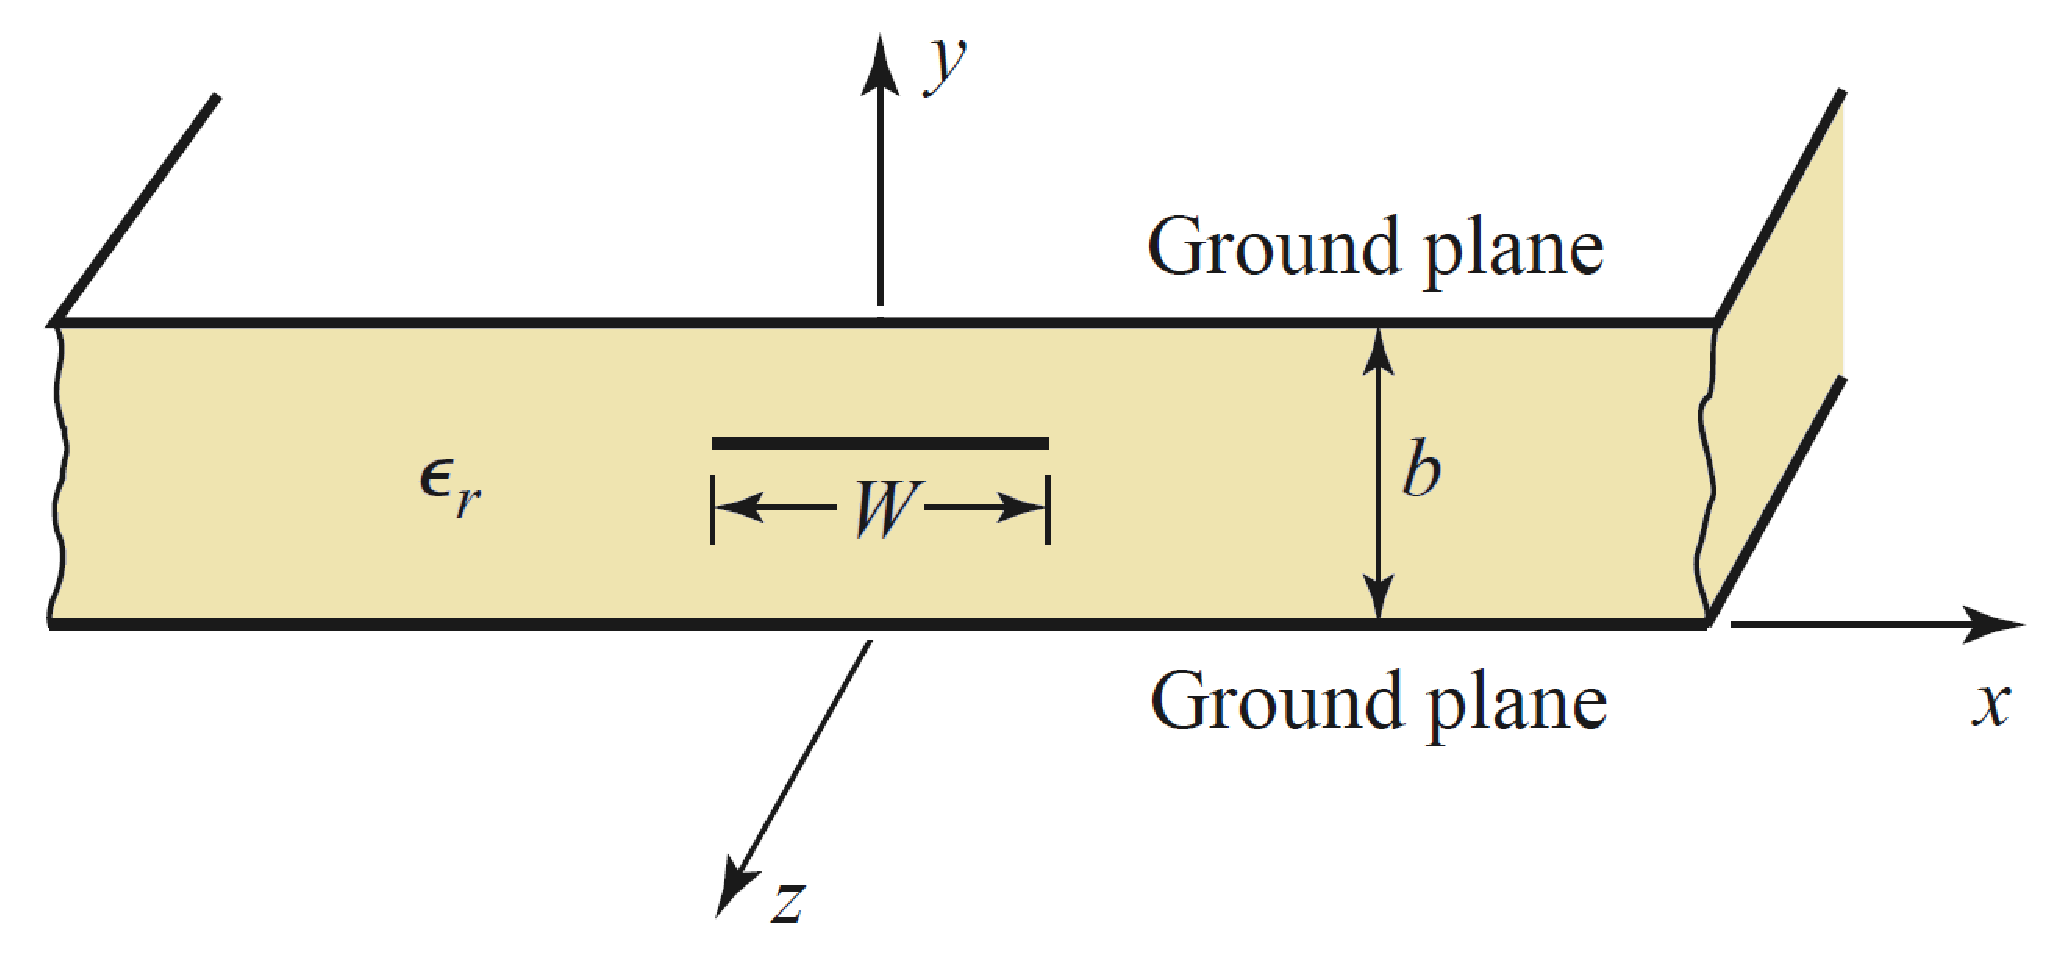
\includegraphics[scale=0.25]{chapter_2/fig3a.eps}\label{th:fig3a} }
\\
\subfloat[] { 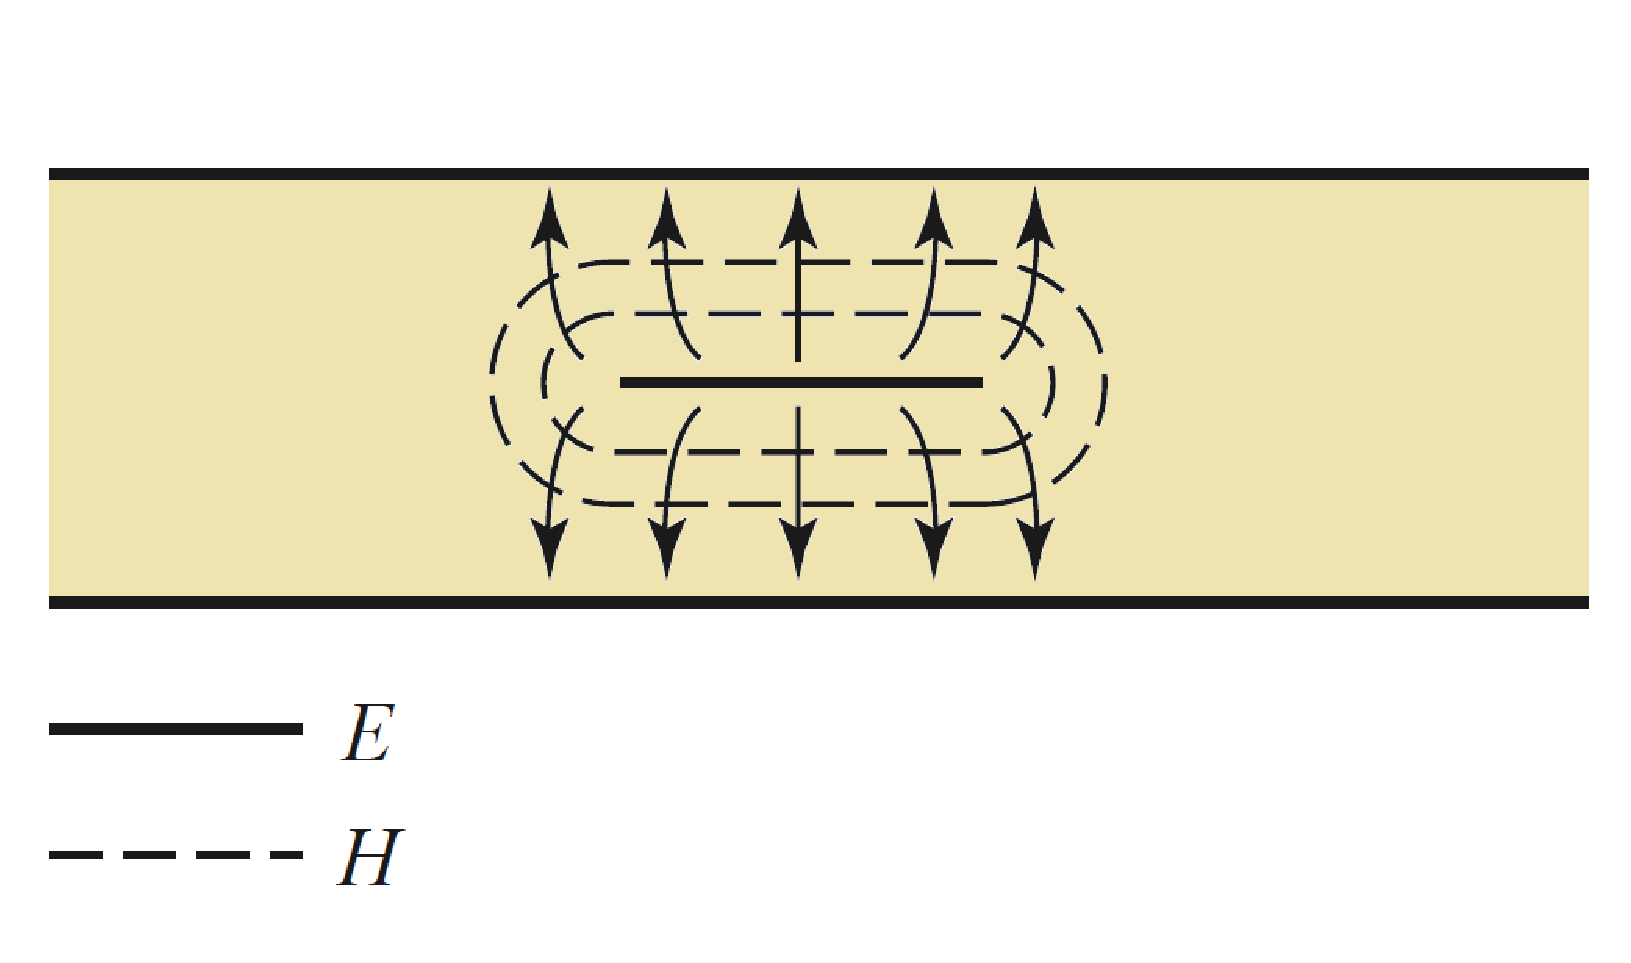
\includegraphics[scale=0.25]{chapter_2/fig3b.eps}\label{th:fig3b} }
\\
\end{tabular}
\caption{Stripline transmission line: geometry (a), electric and magnetic field lines (b).}
\label{th:fig3}
\end{figure}
%%%%%%%%%%%%%%%%%%%%%%%%%%%%%%%%%%%%%%%%%%%%%%%%%%%%%%%%%%%%%

\indent The geometry of stripline is shown in Fig. \ref{th:fig3} together with a sketch of the field lines.  A thin conducting strip of width $W$ is centered between two wide conducting ground planes of separation $b$, and the region between the ground planes is filled with a dielectric material. In practice stripline is usually constructed by etching the center conductor on a grounded dielectric substrate of thickness $b/2$ and then covering with another grounded substrate. Variations of the basic geometry presented in Fig. \ref{th:fig3} include stripline with different dielectric substrate thicknesses (asymmetric stripline) or different dielectric constants (inhomogeneous stripline). Air dielectric is sometimes used when it is necessary to minimize loss.
\\
\indent Since stripline has two conductors and a homogeneous dielectric, it supports a TEM wave, and this is the usual mode of operation. However, stripline can also support higher order waveguide modes. These can usually be avoided in practice by restricting both the ground plane spacing and the sidewall width to less than $\lambda _{d} /2$. Shorting vias between the ground planes are often used to enforce this condition relative to the sidewall width. Shorting vias should also be used to eliminate higher order modes that can be generated when an asymmetry is introduced between the ground planes (e.g., when a surface-mounted coaxial transition is used). A stripline can be considered in a way to be similar to a coaxial transmission line — both have a center conductor completely enclosed by an outer conductor and are uniformly filled with a dielectric medium. 
\\
\indent Because TEM mode of stripline is of primary concern, an electrostatic analysis is sufficient to give the propagation constant and characteristic impedance. Phase velocity can be expressed as:

\begin{equation}\label{th:eq26}
v_{p}=\frac{1}{\sqrt{\mu _{0}\epsilon _{0}\epsilon _{r}}}=\frac{c}{\epsilon _{r}},
\end{equation}

\noindent where $c$ is the speed of light in free-space, and thus the propagation constant of stripline is:

\begin{equation}\label{th:eq27}
\beta =\frac{\omega}{v_{p}}=\omega \sqrt{\mu _{0}\epsilon _{0}\epsilon _{r}}=\sqrt{\epsilon _{r}}k_{0}.
\end{equation}

\noindent The characteristic impedance of a transmission line can be determined under the assumption of very low loss as:

\begin{equation}\label{th:eq28}
Z_{0} =\sqrt{\frac{L}{C}}=\frac{\sqrt{LC}}{C}=\frac{1}{v_{p}C},
\end{equation}

\noindent where $L$ and $C$ are the inductance and capacitance per unit length of the line. Thus, $Z_0$ can be found when knowing $C$.
\\
\indent Since stripline is a TEM line, the attenuation due to dielectric loss can be determined as 

\begin{equation}\label{th:eq29}
\alpha _{d}=\frac{\beta tan\delta }{2} \quad  [Np/m]
\end{equation}

\noindent The attenuation due to conductor loss can be found by the perturbation method or Wheeler’s incremental inductance rule \cite{pozar}. An approximate result is:

\begin{equation}\label{th:eq30}
  \alpha _{c} =
  \begin{cases}
    \frac{2.7x10^{-3}R_{S}\epsilon _{r}Z_{0}}{30\pi (b-t)}A & for\ \sqrt{\epsilon _{r}}Z_{0} < 120\ \Omega \\
    \frac{0.16R_{S}}{Z_{0}b}B  & for\ \sqrt{\epsilon _{r}}Z_{0} > 120\ \Omega
  \end{cases}
 [Np/m]
\end{equation}

\noindent with:

\begin{subequations}\label{th:eq31}
\begin{equation}\label{th:eq31a}
A=1+\frac{W2}{b-t}+\frac{1}{\pi}\frac{b+t}{b-t}ln(\frac{2b-t}{t}),
\end{equation}
\begin{equation}\label{th:eq31b}
B=1+\frac{b}{0.5W+0.7t}(0.5+\frac{0.414t}{W}+\frac{1}{2\pi}ln\frac{4\pi W}{t})
\end{equation}
\end{subequations}

\noindent where $t$ is the thickness of the strip.
\\
% MICROSTRIP

%%%%%%%%%%%%%%%%%%%%%%%%%%%%%%%%%%%%%%%%%%%%%%%%%%%%%%%%%%%%%
\begin{figure}[H]
\centering
\begin{tabular}{c}
\subfloat[] { 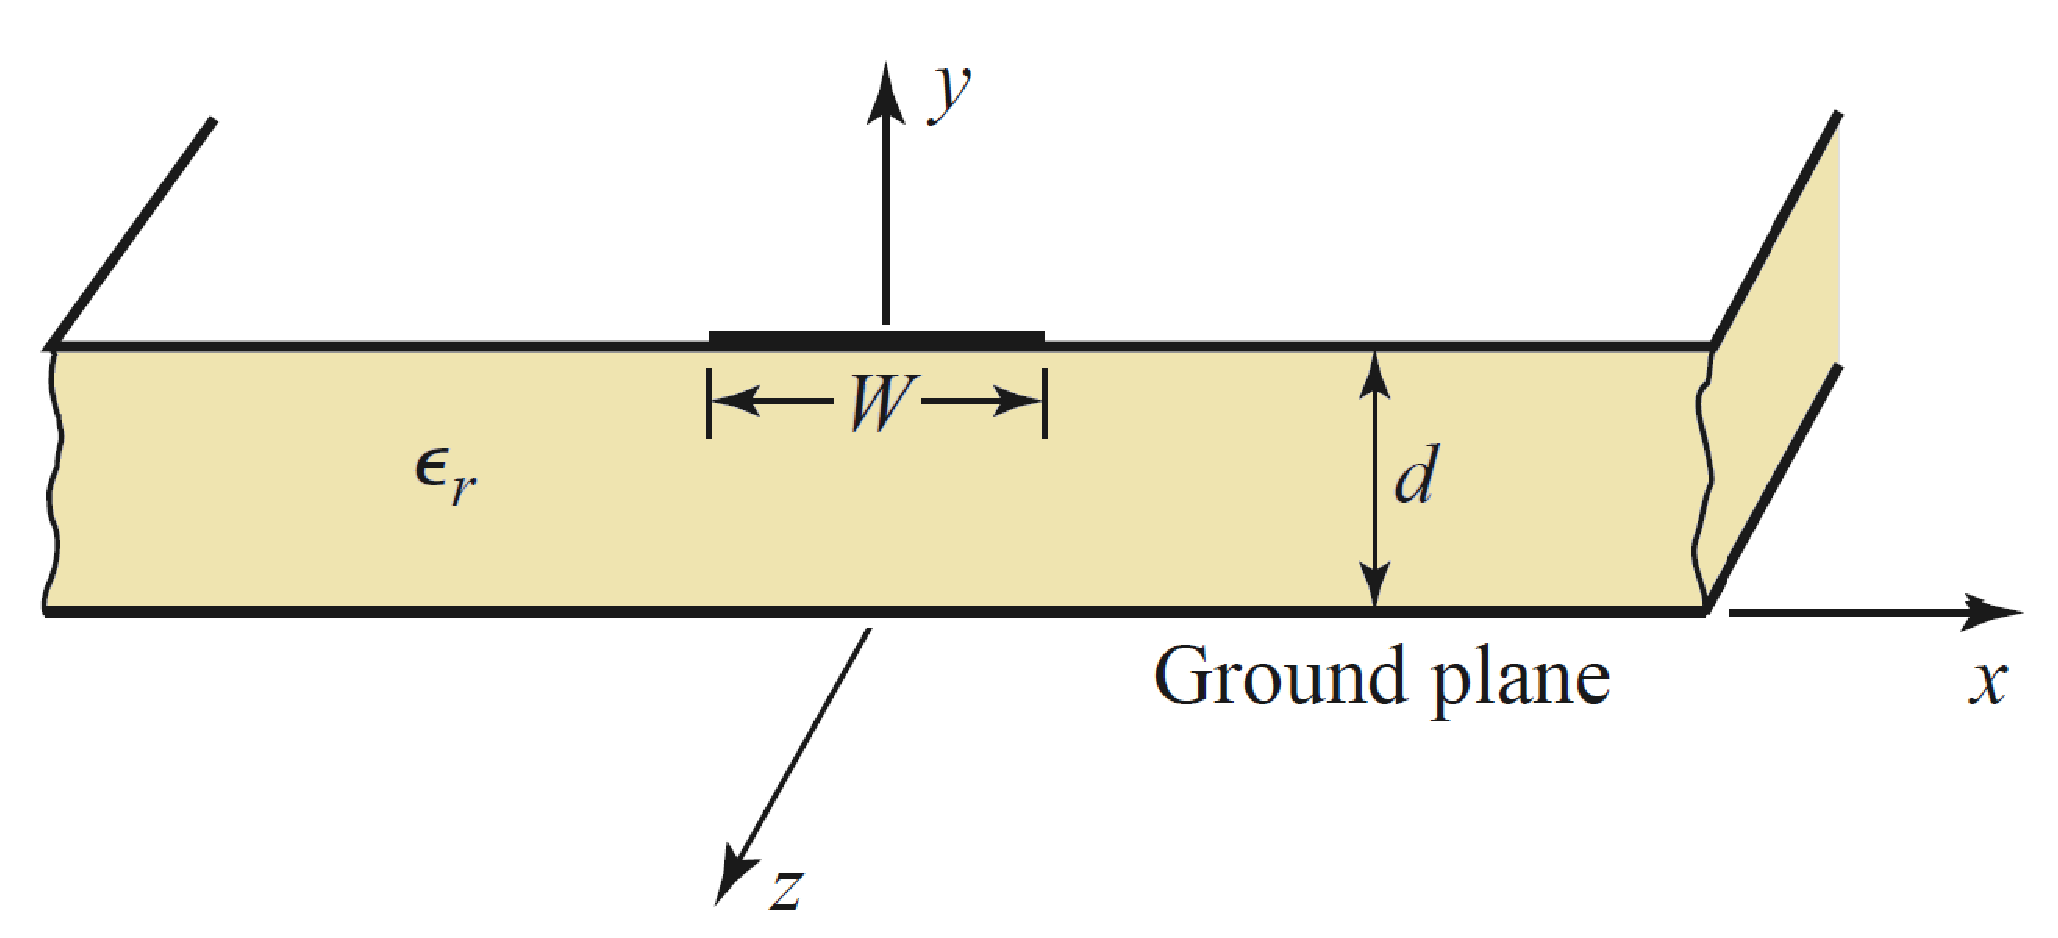
\includegraphics[scale=0.25]{chapter_2/fig4a.eps}\label{th:fig4a} }
\\
\subfloat[] { 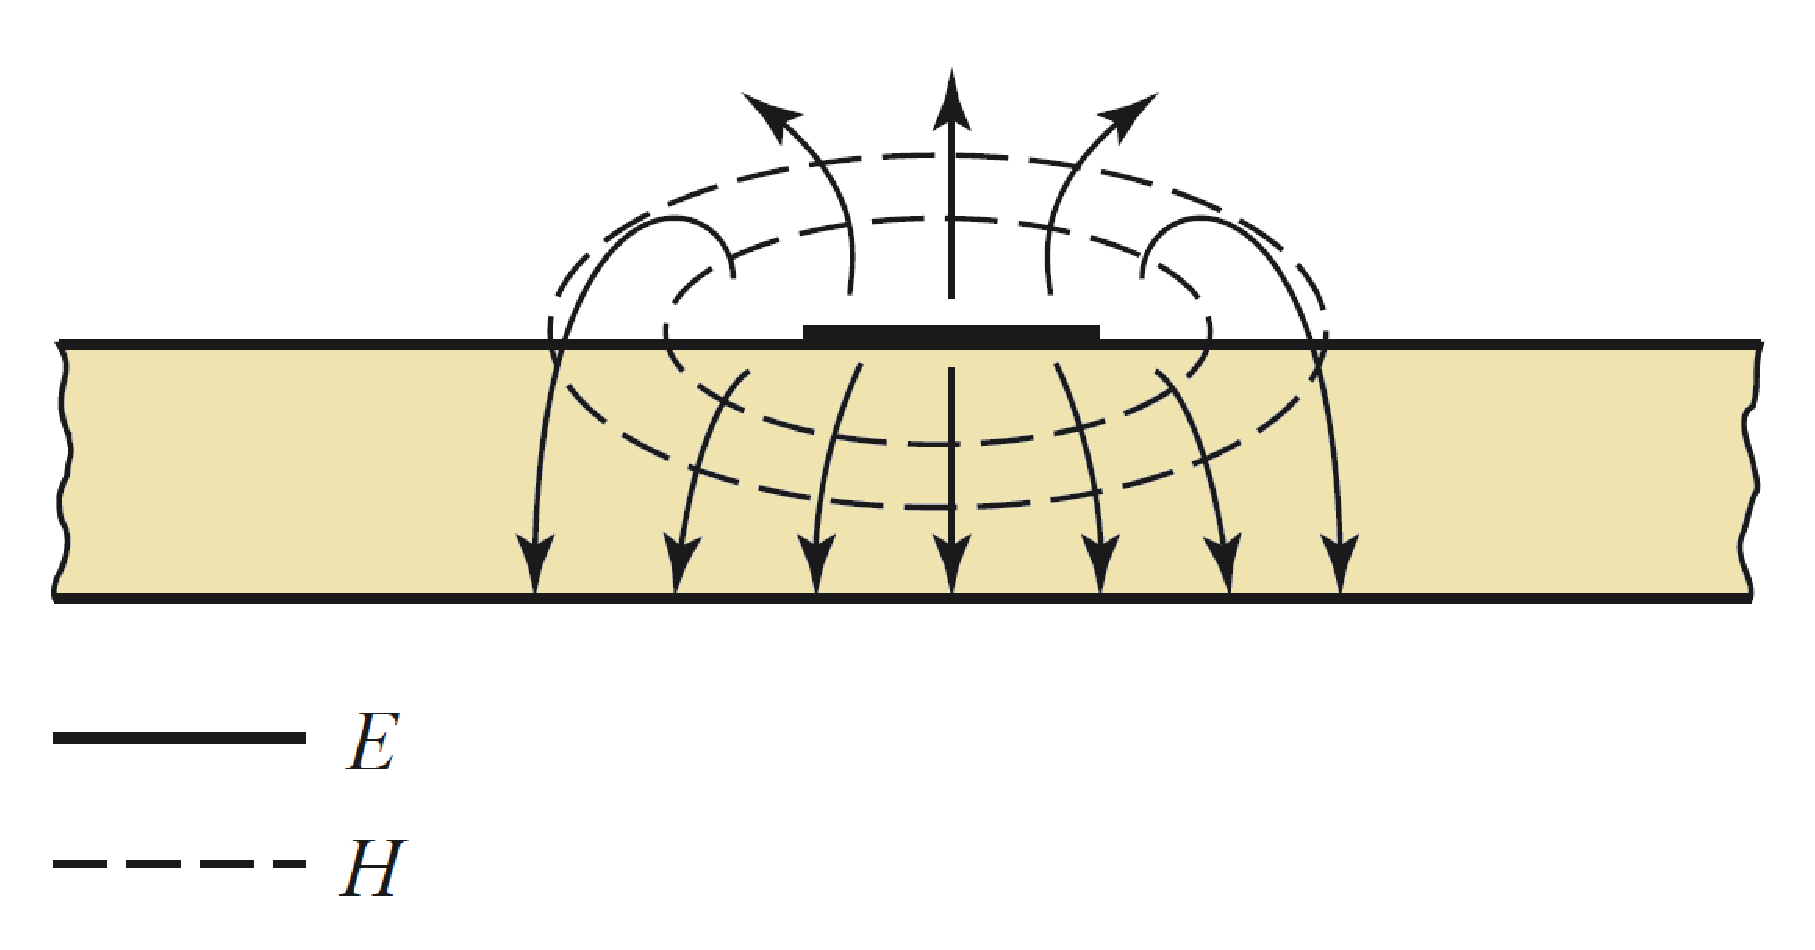
\includegraphics[scale=0.25]{chapter_2/fig4b.eps}\label{th:fig4b} }
\\
\end{tabular}
\caption{Microstrip transmission line: geometry (a), electric and magnetic field lines (b). }
\label{th:fig4}
\end{figure}
%%%%%%%%%%%%%%%%%%%%%%%%%%%%%%%%%%%%%%%%%%%%%%%%%%%%%%%%%%%%%

\indent The geometry of a microstrip line is shown in Fig. \ref{th:fig4} together with a sketch of the field lines. The conductor of width $W$ is printed on a thin, grounded dielectric substrate of thickness $d$ and relative permittivity $\epsilon _{r}$. 
\\
\indent If the dielectric substrate were not present ($\epsilon _{r}$ = 1), microstrip would be a two-wire line consisting of a flat strip conductor over a ground plane, embedded in a homogeneous medium (air). This would constitute a simple TEM transmission line with phase velocity $v_{p} = c$ and propagation constant $\beta = k_0$. 
\\
\indent The presence of the dielectric, particularly the fact that the dielectric does not fill the region above the strip ($y$ > $d$), complicates the behavior and analysis of a microstrip line. Unlike stripline, where all the fields are contained within a homogeneous dielectric region, microstrip has some (usually most) of its field lines in the dielectric region between the strip conductor and the ground plane and some fraction in the air region above the substrate. For this reason microstrip line cannot support a pure TEM wave since the phase velocity of TEM fields in the dielectric region would be $c/\sqrt{\epsilon _{r}}$, while the phase velocity of TEM fields in the air region would be $c$, so a phase-matching condition at the dielectric–air interface would be impossible to enforce.
\\
\indent In actuality, the exact fields of a microstrip line constitute a hybrid TM-TE wave and require more advanced analysis techniques. In most practical applications, however, the dielectric substrate is electrically very thin ($d \ll \lambda $), and so the fields are quasi-TEM. In other words, the fields are essentially the same as those of the static (DC) case. Thus, good approximations for the phase velocity, propagation constant, and characteristic impedance can be obtained from static, or quasi-static, solutions.
Then the phase velocity and propagation constant can be expressed as:

\begin{equation}\label{th:eq32}
v_{p}=\frac{c}{\sqrt{\epsilon _{e}}},
\end{equation}

\begin{equation}\label{th:eq33}
\beta = k_{0}\sqrt{\epsilon _{e}},
\end{equation}

\noindent where $\epsilon _{e}$ is the effective dielectric constant of the microstrip line. Because some of the
field lines are in the dielectric region and some are in the air, the effective dielectric constant satisfies the relation:

\begin{equation}\label{th:eq34}
1 < \epsilon _{e} < \epsilon _{r}
\end{equation}

\noindent and depends on the substrate dielectric constant, the substrate thickness, the conductor
width, and the frequency. The effective dielectric constant of a microstrip line is given approximately by:

\begin{equation}\label{th:eq35}
\epsilon _{e}=\frac{\epsilon _{r}+1}{2}+\frac{\epsilon _{r}-1}{2}\frac{1}{\sqrt{1+12d/W}}.
\end{equation}

\noindent The effective dielectric constant can be interpreted as the dielectric constant of a homogeneous medium that equivalently replaces the air and dielectric regions of the microstrip line. The phase velocity and propagation constant are then given by \ref{th:eq25} and \ref{th:eq26}.
\\
\indent Considering a microstrip line as a quasi-TEM line, the attenuation due to dielectric loss can be determined as:

\begin{equation}\label{th:eq36}
\alpha _{d}=\frac{k_{0}\epsilon _{r}(\epsilon _{e}-1)tan\delta}{2\sqrt{\epsilon _{e}}(\epsilon _{r} -1)} \quad [Np/m],
\end{equation}

\noindent where tan$\delta $ is the loss tangent of the dielectric. The above provided formula account for the fact that the fields around the microstrip line are partially in air (lossless) and partially in the dielectric (lossy). The attenuation due to conductor loss is given approximately by

\begin{equation}\label{th:eq37}
\alpha _{c}=\frac{R_{S}}{Z_{0}W} \quad  [Np/m].
\end{equation}

\noindent For most microstrip substrates, conductor loss is more significant than dielectric loss. Exceptions may occur, however, with some semiconductor substrates.

\cleardoublepage